\chapter{Accommodating QuDs: Qtrees}\label{chap:accommodating-quds}

\textbf{Abstract.} This Chapter introduces a model of questions that is more sophisticated than standardly assumed (cf. Chapter \ref{chap:introduction}). Questions are defined as recursive partitions, or parse trees of the Context Set. This model is shown to capture fine-grained information about how questions relate to each other in terms of specificity, and what it means to answer a question. The Chapter then describes how such questions can be ``retro-engineered'' from assertions, in a compositional way--relatively similarly to the \textit{Dynamic Semantics} framework. Lastly, we suggest ways in which this more fine-grained model of questions can eventually make more fine-grained predictions in the domain of pragmatic oddness. 


\section{Making sense}

\subsection{Oddness despite relevance and informativeness}
In Chapter \ref{chap:introduction}, we have seen that assertive sentences should be informative, i.e. lead to an incremental shrinkage of the Context Set (\textbf{CS}) \citep{Stalnaker1978,Heim1982}. We have also seen that they should be relevant, i.e. shrink the CS in a way consistent with what the Question under Discussion (\textbf{QuD}) is \citep{Lewis1988,Roberts2012}. But sometimes, it is unclear what the QuD should be, and how relevance could help. The follow-up sentences in (\ref{ex2:followups}) exemplify this.

\begin{exe}
	\ex {--Have you seen Jo today?\\
		--No I haven't...}
	\begin{xlist}
		\ex[\#] {I heard she is at a conference in Paris or France.}\label{ex2:hurford-followup}
		\ex[] {Either she is sick, or if she's not sick, she is at a conference.}\label{ex2:non-red-followup}
		\ex[\#] {Either she is sick, or if she's not at a conference, she is sick.}\label{ex2:red-followup}
	\end{xlist} \label{ex2:followups}
\end{exe}

In these answers, the explicit question \textit{Have you seen Jo today?} is first settled, so that there is not explicit QuD left to be addressed. Yet, it appears that the follow-up assertions address a different question, along the lines of \textit{Where is Jo?}. But how exactly this question gets derived from the sentences at stake, remains unclear. Additionally, not all follow-up sentences appear felicitous. (\ref{ex2:hurford-followup}) instantiates a Hurford Disjunction \citep{Hurford1974}, i.e., at the descriptive level, a disjunction whose disjuncts are in a relation of contextual entailment (\textit{Paris} $\vdash$ \textit{France}). This disjunction is informative: it says that \textit{Jo is at a conference in France}. It is also relevant to the question that gets intuitively inferred from the exchange: it identifies an event and a country where Jo is at the moment. Yet, (\ref{ex2:hurford-followup}) is sharply odd. There are in fact many successful accounts of (\ref{ex2:hurford-followup})'s oddness, building on constraints independent of the QuD and \textsc{Relevance}.

But we will see in Chapter \ref{chap:redundancy} that such accounts fall short in explaining the contrast between (\ref{ex2:non-red-followup}) and (\ref{ex2:red-followup}). These two follow-up sentences are both informative: assuming implication is material, they both mean that Jo is sick or at a conference. They also appear intuitively relevant to a QuD along the lines of \textit{Where is Jo?}. Yet, (\ref{ex2:non-red-followup}) makes perfect sense, while (\ref{ex2:red-followup}) does not seem to make any sense. The goal is then to devise a pragmatic model of these sentences in which (i) they package information differently, and (ii) unlike (\ref{ex2:hurford-followup}) and (\ref{ex2:red-followup}), (\ref{ex2:non-red-followup}), packages information in a way that is pragmatically optimal.

\subsection{Overview  and motivation of the Chapter}
The machinery we introduce in this Chapter aims to account the above datapoints (among others), by relating the oddness of the follow-ups in (\ref{ex2:hurford-followup}) and (\ref{ex2:red-followup}) to the QuD(s) inferred from them. The fundamental principle we want to operationalize is \textit{Question-Answer Congruence} (henceforth \textbf{QAC}), repeated in (\ref{ex2:q-a-congruence}). 

\begin{exe}
	\ex {\textit{Question-Answer Congruence (\textbf{QAC}, \citenp{Katzir2015}).} A felicitous assertion has to be a good answer to a good question.}\label{ex2:q-a-congruence}
\end{exe}

Chapter \ref{chap:introduction} showed that \textsc{Relevance} could rule out a wide range of question-answer pairs, and as such could constitute a partial implementation of QAC. The dissertation will show that, under a certain interpretation of ``good answer'' and ``good question'', many more cases of pragmatic oddness can be understood as an accross-the-board failure of QAC.

In ths Chapter, we will lay out the groundwork for this analysis, by first introducing a more sophisticated model of questions, based on recursive partitions or trees, instead of mere partitions of the CS. This model is building on \citet{Buring2003,Ippolito2019,Zhang2022}, among many others. Additionally, we will suggest that questions can be evoked by assertions in a compositional way, such that more complex sentence tend to give rise to more structurally complex questions, and also, such that sentences involving different operators (specifically, disjunctions and conditionals), give rise to different kinds of questions. In this model, each sentence may be associated with multiple potential questions. In line with QAC, a sentence which cannot be felicitously paired with \textit{any} question will be deemed odd. This can happen if \textit{all} the pairs formed by a sentence and a question it evokes, are themselves ill-formed. This Chapter will focus on what it takes to get there: how questions should be modeled, and how question-answer pairs are generated from simple and more complex sentences. Chapters \ref{chap:redundancy} and \ref{chap:relevance} will introduce specific constraints on question-answer pairs allowing to capture data like (\ref{ex2:followups}).


This kind of machinery is independently motivated by the idea that sentences are never uttered in and of themselves; their purpose is to answer a question, overt or not, and to induce further questions \cite{Roberts1996}. A pragmatic model of assertion therefore needs to integrate what sentences mean, but also what kind of information structure they evoke. Unlike inquisitive semantics \citep{Mascarenhas2008,Ciardelli2009,Groenendijk2009,Ciardelli2018}, which proposes an \textit{unified} view of questions and assertions at the semantic level, what we propose here is a form of inquisitive \textit{pragmatics}: sentences are still assigned ``standard'' extensional/intensional meaning, but also have an inquisitive contribution at the pragmatic level. In fact, the current machinery may be closer in spirit to Dynamic Semantics \citep{Heim1983a,Heim1983b}, where different operators give rise to different incremental updates of the Context Set. Under our view, different operators will give rise to different \textit{parses} of the Context Set, at the inquisitive level. This will eventually allow to capture a contrast between (\ref{ex2:red-followup}) and (\ref{ex2:non-red-followup}). On top of this model, Chapters \ref{chap:redundancy} and \ref{chap:relevance} will introduce constraints on pairs formed by sentences and their accommodated questions, allowing to capture the oddness of e.g. (\ref{ex2:hurford-followup}) and (\ref{ex2:red-followup}). Chapter \ref{chap:redundancy} will discuss (\ref{ex2:non-red-followup}), (\ref{ex2:red-followup}), and variants thereof, arguing that some, but crucially not all variants, appear redundant once inferred QuDs are taken into consideration. Chapter \ref{chap:redundancy} will also cover the case of (\ref{ex2:hurford-followup}), and some of its variants.

We now proceed to define questions, not just as partition, but rather, as parse trees of the Context Set, that we will call Qtrees.

\section{Structure of Question Trees}

\subsection{From partitions to recursive partitions, to parse trees}
Building on the standard model presented in Chapter \ref{chap:introduction}, we introduce a more sophisticated view of the pragmatics of questions. This model will incorporate the idea that questions have internal structure, and specifically, are hierarchically organized. A question such as (\ref{ex2:city-question}) for instance, appears more \textit{fine-grained}, than a question like (\ref{ex2:country-question}). Alternatively, whatever proposition identifies a cell in (\ref{ex2:city-question}), also identifies a cell in (\ref{ex2:city-question}). This will be accounted for, as part of the internal structure of questions.

\begin{exe}
	\ex 
	\begin{xlist}
		\ex {In which city did Jo grow up?}\label{ex2:city-question}
		\ex {In which country did Jo grow up?}\label{ex2:country-question}
	\end{xlist}
\end{exe}

First, let us observe these intuitions about question specificity are \textit{not} readily cashed out by standard partitions or alternative set associated with questions. In the case of (\ref{ex2:city-question}) and (\ref{ex2:country-question}), these two notions coincide--\textit{modulo} intersection with the CS. In partition talk, (\ref{ex2:city-question}) induces a by-city partition of the CS (see (\ref{ex2:city-partition}) and Figure \ref{fig2:city-partition}), while (\ref{ex2:country-question}) induces a by-country partition (see (\ref{ex2:country-partition}) and Figure \ref{fig2:country-partition}). But nothing in (\ref{ex2:city-question})'s partition signals that each of its cells is properly contained in a cell of (\ref{ex2:country-question})'s partition. This property can de derived from the two structures, but is not readily \textit{encoded} by them.

\begin{exe}
	\ex 
	\begin{xlist}
		\ex {$\llbracket$ In which city did Jo grow up?$\rrbracket^w$ =\\$\lbrace p \ | \ \exists l. \ \text{$l$ is a city} \wedge p = \lambda w'. \ \text{Jo grew up in $l$ in $w'$}\rbrace$}\label{ex2:city-partition}
		\ex {$\llbracket$ In which country did Jo grow up?$\rrbracket^w$ =\\$\lbrace p \ | \ \exists l. \ \text{$l$ is a country} \wedge p = \lambda w'. \ \text{Jo grew up in $l$ in $w'$}\rbrace$}\label{ex2:country-partition}
	\end{xlist}
\end{exe}

\begin{figure}[H]
	\centering
	\begin{subfigure}[t]{.48\linewidth}
		\centering
		\scalebox{1.25}{
		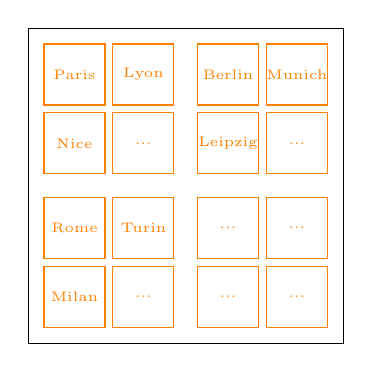
\begin{tikzpicture}	
			\draw [draw=black] (0, 0) rectangle (4,4) ;
			\draw [draw=orange] (0.2, 2.15) rectangle (0.975, 2.925) node[pos=.5] {\tiny \textcolor{orange}{Nice}};
			\draw [draw=orange] (1.075, 2.15) rectangle (1.85, 2.925) node[pos=.5] {\tiny \textcolor{orange}{...}};
			\draw [draw=orange] (0.2, 3.025) rectangle (0.975, 3.8) node[pos=.5] {\tiny \textcolor{orange}{Paris}};
			\draw [draw=orange] (1.075, 3.025) rectangle (1.85, 3.8) node[pos=.5] {\tiny \textcolor{orange}{Lyon}};
			\draw [draw=orange] (0.2, 0.2) rectangle (0.975, 0.975) node[pos=.5] {\tiny \textcolor{orange}{Milan}};
			\draw [draw=orange] (1.075, 0.2) rectangle (1.85, 0.975) node[pos=.5] {\tiny \textcolor{orange}{...}};
			\draw [draw=orange] (0.2, 1.075) rectangle (0.975, 1.85) node[pos=.5] {\tiny \textcolor{orange}{Rome}};
			\draw [draw=orange] (1.075, 1.075) rectangle (1.85, 1.85) node[pos=.5] {\tiny \textcolor{orange}{Turin}};
			
			\draw [draw=orange] (2.15, 0.2) rectangle (2.925, 0.975) node[pos=.5] {\tiny \textcolor{orange}{...}};
			\draw [draw=orange] (3.025, 0.2) rectangle (3.8, 0.975) node[pos=.5] {\tiny \textcolor{orange}{...}};
			\draw [draw=orange] (2.15, 1.075) rectangle (2.925, 1.85) node[pos=.5] {\tiny \textcolor{orange}{...}};
			\draw [draw=orange] (3.025, 1.075) rectangle (3.8, 1.85) node[pos=.5] {\tiny \textcolor{orange}{...}};
			
			\draw [draw=orange] (2.15, 2.15) rectangle (2.925, 2.925) node[pos=.5] {\tiny \textcolor{orange}{Leipzig}};
			\draw [draw=orange] (3.025, 2.15) rectangle (3.8, 2.925) node[pos=.5] {\tiny \textcolor{orange}{...}};
			\draw [draw=orange] (2.15, 3.025) rectangle (2.925, 3.8) node[pos=.5] {\tiny \textcolor{orange}{Berlin}};
			\draw [draw=orange] (3.025, 3.025) rectangle (3.8, 3.8) node[pos=.5] {\tiny \textcolor{orange}{Munich}};
		\end{tikzpicture}}
		\caption{By-city partition associated with (\ref{ex2:city-partition}). Cells are ordered on a grid for clarity only.}\label{fig2:city-partition}
	\end{subfigure}\hfill
	\begin{subfigure}[t]{.48\linewidth}
		\centering
		\scalebox{1.25}{
		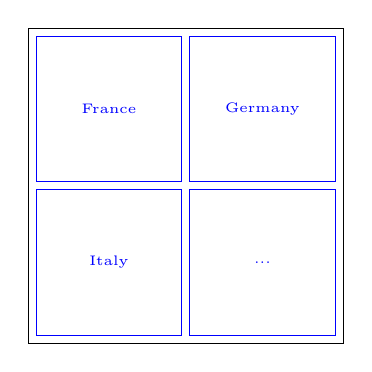
\begin{tikzpicture}	
			\draw [draw=black] (0, 0) rectangle (4,4);
			\draw [draw=blue] (0.1, 2.05) rectangle (1.95, 3.9) node[pos=.5] {\tiny \textcolor{blue}{France}};
			\draw [draw=blue] (2.05, 0.1) rectangle (3.9, 1.95) node[pos=.5] {\tiny \textcolor{blue}{...}};
			\draw [draw=blue] (0.1, 0.1) rectangle (1.95, 1.95) node[pos=.5] {\tiny \textcolor{blue}{Italy}};
			\draw [draw=blue] (2.05, 2.05) rectangle (3.9, 3.9) node[pos=.5] {\tiny \textcolor{blue}{Germany}};
		\end{tikzpicture}}
		\caption{By-country partition associated with (\ref{ex2:country-partition}). Cells are ordered on a grid for clarity only.}
	\end{subfigure}
	\caption{Standard partitions induced by a fine-grained (\ref{ex2:city-partition}) and a coarser-grained question (\ref{ex2:country-partition}).}\label{fig2:country-partition}
\end{figure}

Intuitively, adding ``brackets'' to (\ref{ex2:city-partition}) grouping together propositions talking about cities belonging to the same country, would help capture the desired property. This is done in (\ref{ex2:city-parse}). (\ref{ex2:city-parse}) then defines a set of sets of propositions. 
\begin{exe}
	\ex {$\llbracket$ In which city did Jo grow up?$\rrbracket^w$ =\\$\lbrace\lbrace p \ | \ \exists l. \ \text{$l$ is a city in $l'$} \wedge \ p = \lambda w'. \ \text{Jo grew up in $l$ in $w'$}\rbrace \ | \ l' \text{ is a country} \rbrace$}\label{ex2:city-parse}
\end{exe}

Grouping together cells within bigger sets (which are cells themselves), amounts to building a \textit{recursive} partition of the CS. In our example, the ``outer'' partition is by-country, and the ``inner'' partition, is by-city. Graphically, this is equivalent to adding the ``blue rectangles'' from Figure \ref{fig2:country-partition}, to Figure \ref{fig2:city-partition}. This operation is performed in Figure \ref{fig2:city-recursive-partition}. The tree in Figure \ref{fig2:city-tree} is yet another, more readable way to represent the same thing. In this tree, each node refers to a proposition of the form \textit{Jo grew up in l}, $l$ denoting a city or a country. Each node is understood as intersected with the CS, which corresponds to the root of the tree. Nodes appearing at the same level (forming a ``layer''),partition the CS. Deeper layers, correspond to finer-grained partitions.

\begin{figure}[H]
	\centering
	\begin{subfigure}[t]{.45\linewidth}
		\centering
		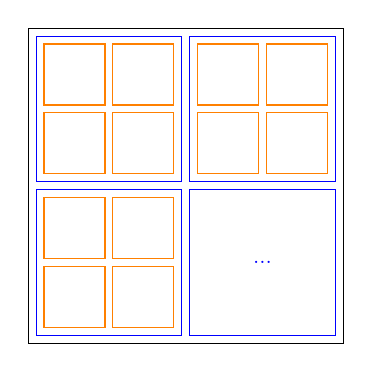
\begin{tikzpicture}	
			\draw [draw=black] (0, 0) rectangle (4,4) ;
			\draw [draw=blue] (0.1, 2.05) rectangle (1.95, 3.9);
				\draw [draw=orange] (0.2, 2.15) rectangle (0.975, 2.925);
				\draw [draw=orange] (1.075, 2.15) rectangle (1.85, 2.925);
				\draw [draw=orange] (0.2, 3.025) rectangle (0.975, 3.8);
				\draw [draw=orange] (1.075, 3.025) rectangle (1.85, 3.8);
			\draw [draw=blue] (2.05, 0.1) rectangle (3.9, 1.95) node[pos=.5] {\scriptsize \textcolor{blue}{...}};
			\draw [draw=blue] (0.1, 0.1) rectangle (1.95, 1.95);
				\draw [draw=orange] (0.2, 0.2) rectangle (0.975, 0.975);
				\draw [draw=orange] (1.075, 0.2) rectangle (1.85, 0.975);
				\draw [draw=orange] (0.2, 1.075) rectangle (0.975, 1.85);
				\draw [draw=orange] (1.075, 1.075) rectangle (1.85, 1.85);
			\draw [draw=blue] (2.05, 2.05) rectangle (3.9, 3.9);
				\draw [draw=orange] (2.15, 2.15) rectangle (2.925, 2.925);
				\draw [draw=orange] (3.025, 2.15) rectangle (3.8, 2.925);
				\draw [draw=orange] (2.15, 3.025) rectangle (2.925, 3.8);
				\draw [draw=orange] (3.025, 3.025) rectangle (3.8, 3.8);
		\end{tikzpicture}
		\caption{Recursive partition view}\label{fig2:city-recursive-partition}
	\end{subfigure}
	\hfill
	\begin{subfigure}[t]{.5\linewidth}
		\centering
		\vspace{-4.4cm}
		\begin{forest}
			[{CS\\
				Jo grew up in...}[\textcolor{blue}{France}[\textcolor{orange}{{Paris}}][\textcolor{orange}{Lyon}][\textcolor{orange}{...}]][\textcolor{blue}{Germany}[\textcolor{orange}{Berlin}][\textcolor{orange}{...}]][\textcolor{blue}{Italy}[\textcolor{orange}{...}]][\textcolor{blue}{...}]]
		\end{forest}
		\caption{Tree view}\label{fig2:city-tree}
	\end{subfigure}
	\caption{Alternative representations of the CS corresponding to the nested sets of (\ref{ex2:city-parse}).}\label{tree:country-city-parse}
\end{figure}

(\ref{ex2:set-tree-bijection}) formally defines the bijective mapping between recursive sets of propositions (dubbed \textit{inductive propositions}) like (\ref{ex2:city-parse}), and tree structures like Figure \ref{fig2:city-tree}.
\begin{exe}
	\ex {\textit{Set-to-tree bijection. } To define this bijection, we first define inductive propositions, and their propositional content. $S$ is an inductive proposition if either:
		\begin{itemize}
			\item $S$ is a set of worlds (i.e. a proposition);
			\item $S$ is a set of inductive propositions.
		\end{itemize}
		The propositional content of an inductive proposition is then defined as:
		\begin{itemize}
			\item If $S$ is a proposition: $S$;
			\item If $S$ is a set of inductive propositions: the grand union of the propositional contents of $S$'s elements.
		\end{itemize}
		Any inductive proposition $S$ is in a bijection with a tree structure whose nodes are propositions, and defined as:
		\begin{itemize}
			\item If $S$ is a proposition: the tree node denoting $S$;
			\item If $S$ is a set of inductive propositions: the tree whose root denotes $S$'s propositional content, and whose children are the tree structures induced by each of $S$'s elements. 
	\end{itemize}}\label{ex2:set-tree-bijection}
\end{exe}

We now generalize these observations, which, in fact, are not new. Building on \citet{Buring2003,Riester2019,Onea2016,Ippolito2019,Zhang2022} (among others), we take questions to denote \textit{parse trees} of the CS, i.e. structures that hierarchically organize the worlds of the CS. Such trees (abbreviated \textbf{Qtrees}) are defined in (\ref{ex2:qtree-def}). 
%(\ref{ex2:parse-def}) provide a more general definition of a parse.\footnote{This slightly differs from the notion of parse defined for sentences for instance, in which linear precedence must be preserved.} 
\begin{exe}
	\ex {\textit{Structure of Question-trees (\textbf{Qtrees}).} Qtrees are rooted trees whose nodes are all subsets of the CS and s.t.:
		\begin{itemize}
			\item Their root generally\footnote{In the case of sentences carrying presuppositions, the root will be assumed to correspond to the intersection between the CS and the sentence's presupposition. In fact, the whole Qtree will be nodewise intersected with the presupposition. This will be put to use in Chapters \ref{chap:scalarity} and \ref{chap:exh-incr}. But the examples we will see before this, will all involve Qtree rooted in the CS.} refers to the CS;
			\item Any intermediate node is a proposition, which is partitioned by the set of its children.
		\end{itemize}
	}\label{ex2:qtree-def}
\end{exe}
%	\ex {\textit{Parse.} Let $S$ be a set. A parse of $S$ is a rooted tree whose nodes are subsets of $S$ and s.t.:
%		\begin{itemize}
%			\item The root is $S$;
%			\item Any intermediate node is partitioned by the set of its children.
%		\end{itemize}
%	}\label{ex2:parse-def}

Before investigating the interpretation and the structural properties of this more sophisticated model of questions, the next Section covers a few core concepts from graph theory that will be useful in the rest of the Chapter and beyond.


\subsection{A brief refresher on graph theory (and a few useful concepts for Qtrees)}

(\ref{ex2:qtree-def}) defines questions as rooted trees. Here, we precisify what it means to be a tree, and moreover, what is means to be a \textit{rooted} tree (\ref{ex:rooted-tree}). Let us unpack  (\ref{ex:rooted-tree}), and, first, disregard the ``rooted'' aspect of it. A tree is a kind of graph. A graph is a way to represent a binary relation, which by default will be symmetric (\textit{directed} graphs implement asymmetric relations). Elements in the domain of the relation are modeled as nodes, and unordered pairs of nodes are connected with and edge, iff they verify the relation. A graph therefore amounts to a set of nodes, and a set of edges between these nodes. This is summarized in (\ref{ex:graph}), and illustrated in Figure \ref{fig:basic-graph}.

\begin{exe}
	\ex {\textit{Rooted tree.} A rooted tree is a graph that is connected and acyclic, and features a distinguished node called root.}\label{ex:rooted-tree}
	\ex {\textit{(Undirected) Graph.} An undirected graph (or just a graph) is defined by a set of nodes $\mathcal{N}$ and by a set of edges $\mathcal{E}$ between elements of $\mathcal{N}$. Edges are defined as unordered pairs of nodes: $\mathcal{E} \subseteq \lbrace \lbrace N_1, N_2\rbrace \ | \ (N_1, N_2) \in \mathcal{N}^2\rbrace$}\label{ex:graph}
\end{exe}

\begin{figure}[H]
	\centering
	\begin{tikzpicture}
		\node[shape=circle,draw=black] (A) at (0,0) {A};
		\node[shape=circle,draw=black] (B) at (0,3) {B};
		\node[shape=circle,draw=black] (C) at (2.5,4) {C};
		\node[shape=circle,draw=black] (D) at (2.5,1) {D};
		\node[shape=circle,draw=black] (F) at (5,3) {F} ;
		\node[shape=circle,draw=black] (E) at (-2,2) {E} ;
		
		\path [-] (A) edge node[left] {} (B);
		\path [-](B) edge node[left] {} (C);
		\path [-](A) edge node[left] {} (D);
		\path [-](D) edge node[left] {} (C);
		\path [-](D) edge node[right] {} (F);   
	\end{tikzpicture}
	\caption{An (undirected) graph $G=(\mathcal{N}, \mathcal{E})$, with $\mathcal{N}=\lbrace A, B, C, D, E, F\rbrace$ and $\mathcal{E}=\lbrace \lbrace A, B\rbrace, \lbrace A, D\rbrace, \lbrace B, C\rbrace, \lbrace C, D\rbrace, \lbrace D, F\rbrace\rbrace$.}\label{fig:basic-graph}
\end{figure}

In graphs, sequences of adjacent edges form paths. For instance, in Figure \ref{fig:basic-graph}, the sequence $[\lbrace A, B\rbrace, \lbrace A, D\rbrace, \lbrace D, F\rbrace]$ forms a path, between node $A$ and node $F$. This is generalized in (\ref{ex:graph-path}).

\begin{exe}
	\ex {\textit{Path.} Let $G = (\mathcal{N}, \mathcal{E})$ be a graph. Let $(N_1, N_2) \in \mathcal{N}^2$ be two nodes of $G$. There is a path in $G$ between $N_1$ and $N_2$ (abbreviated $N_1 \stackrel{G}{\leadsto}  N_2$) iff $N_1$ and $N_2$ can be connected by a series of edges in $G$, i.e. $\exists (e_1, ... e_k) \in \mathcal{E}^k. \ N_1 \in e_1 \wedge N_2 \in e_k \wedge \forall i \in [1; k-1]. \  |e_i \cap e_{i+1}|  = 1$, where $|.|$ is the cardinality operator.}\label{ex:graph-path}
\end{exe}

In Figure \ref{fig:basic-graph}, it is easy to see that nodes $A$, $B$, $C$, $D$ and $F$ are all connected to each other by at least one path (in fact, infinitely many of them). Node $E$ on the other hand, is isolated. So, Figure \ref{fig:basic-graph} represents a graph that is \textit{not} connected. If $E$ were removed from the set of nodes, and the edges remained the same, the resulting graph would be connected. This concept of connectivity is generalized in (\ref{ex:graph-connectivity}). If a graph is a tree, then, it is connected.
\begin{exe}
	\ex {\textit{Connectivity.} Let $G = (\mathcal{N}, \mathcal{E})$ be a graph. $G$ is connected, iff there is a path in $G$ between any pair of nodes in $\mathcal{N}$, i.e. $\forall (N_1, N_2) \in \mathcal{N}^2. \ N_1 \stackrel{G}{\leadsto} N_2$.}\label{ex:graph-connectivity}
\end{exe}

Another thing to note about Figure \ref{fig:basic-graph}, is that nodes $A$, $B$, $C$, and $D$ form a ``cycle'', there is a path that starts at one of these nodes (e.g., $C$), and ends at this very same node, \textit{via} $B$, $A$, and $D$. Because of this cycle, there are infinitely many paths between $A$, $B$, $C$, and $D$, and also between each of these nodes, and $F$. Removing the edge between, say, $A$ and $B$, would break the cycle (yet, interestingly, maintain connectivity between $A$, $B$, $C$, and $D$). The resulting graph would be acyclic. The general definition of an acyclic graph, is given in (\ref{ex:graph-acyclic}). If a graph is a tree, then, it is acyclic. Moreover, connectivity and acyclicity, are necessary and sufficient for a graph to be a tree.

\begin{exe}
	\ex {\textit{Acyclicity.} Let $G = (\mathcal{N}, \mathcal{E})$ be a graph. $G$ is acyclic, iff no node $N$ of $\mathcal{N}$ is s.t. there is a path starting and ending at $N$ in $G$, i.e. $\neg\exists N \in \mathcal{N}. \ N \stackrel{G}{\leadsto} N$.}\label{ex:graph-acyclic}
\end{exe}

We now have a definition of what kind of data structure a tree is. But why do we need  Qtrees to be ``rooted'' then? To understand why, let us go back to the tree in Figure \ref{fig2:city-tree}, repeated in Figure \ref{fig2:city-tree-repeated} below. The way this tree is represented on paper, is somehow misleading. Recall that a tree is just an undirected graph, with a few extra properties constraining its edges. If Figure \ref{fig2:city-tree-repeated} were not ``rooted'', nothing would prevent us to represent it in the form of Figure \ref{fig2:city-tree-france-root}: the nodes and edges are strictly the same, but in Figure \ref{fig2:city-tree-france-root}, \textit{France} ``appears'' to be the root of the tree, because it is represented at the top. To avoid this confusion, the fact that the CS node should be ``at the top'' is made part of the representation of the tree--which then becomes a \textit{rooted} tree. So, a rooted tree is just a tree, plus one distinguished node that serves as root.

\begin{figure}[H]
	\centering
	\begin{subfigure}[t]{.45\linewidth}
		\centering
		\begin{forest}
			[{CS\\
				Jo grew up in...}[\textcolor{blue}{France}[\textcolor{orange}{{Paris}}][\textcolor{orange}{Lyon}][\textcolor{orange}{...}]][\textcolor{blue}{Germany}[\textcolor{orange}{Berlin}][\textcolor{orange}{...}]][\textcolor{blue}{Italy}[\textcolor{orange}{...}]][\textcolor{blue}{...}]]
		\end{forest}
		\caption{Tree view of (\ref{ex2:city-question})}\label{fig2:city-tree-repeated}
	\end{subfigure}
	\hfill
	\begin{subfigure}[t]{.45\linewidth}
		\centering
		\begin{forest}
			[\textcolor{blue}{France}[\textcolor{orange}{Paris}][\textcolor{orange}{Lyon}][\textcolor{orange}{...}][CS[\textcolor{blue}{Germany}[\textcolor{orange}{Berlin}][\textcolor{orange}{...}]][\textcolor{blue}{Italy}[\textcolor{orange}{...}]][\textcolor{blue}{...}]]]
		\end{forest}
		\caption{Alternative tree view of (\ref{ex2:city-question}), assuming Qtrees were not rooted}\label{fig2:city-tree-france-root}
	\end{subfigure}
\end{figure}


The notion of a distinguished root in fact allows to define a few interesting properties on trees, that will be used throughout the dissertation. First, once a tree is rooted, it is possible to define a measure of distance between each node of the tree, and the root. This is the concept of depth defined in (\ref{ex:tree-node-depth}). In Figure \ref{fig2:city-tree-repeated} for instance, the CS has depth $0$, \textit{Germany} depth $1$, and \textit{Lyon} depth $2$. This also allows to define the global ``size'' of the tree, in the form of its maximal depth; see (\ref{ex:tree-depth}). Figure \ref{fig2:city-tree-repeated} for instance, is a tree of depth $2$.

\begin{exe}
	\ex
	\begin{xlist}	
		\ex {\textit{Depth of a node in a rooted tree.} Let $T = (\mathcal{N}, \mathcal{E}, R)$ be a rooted tree, with root $R$. Let $N \in \mathcal{N}$. The depth of $N$ in $T$ ($d(N, T)$) corresponds to the length of the minimal path between $R$ and $N$ if $N \neq R$,\footnote{This path can be determined using a simple Depth-First Search algorithm starting from the root.} and is set to $0$ if $N = R$.}\label{ex:tree-node-depth}
		\ex {\textit{Depth of a rooted tree.} Let $T = (\mathcal{N}, \mathcal{E}, R)$ be a rooted tree, with root $R$. The depth of $T$ ($d(T)$) is the maximal depth of a node in $T$: $d(T) = max_{N \in \mathcal{N}}(d(N, T))$.}\label{ex:tree-depth}
	\end{xlist}
\end{exe}

Lastly, we will extensively use the concept of \textit{layer}, that we define as a the maximal set of same-depth nodes in a rooted tree; see (\ref{ex:tree-layer}). Figure \ref{fig2:city-tree-repeated} features a country-layer at depth $1$, and a city-layer at depth $2$. Layers therefore reflect an intuitive notion of granularity.

\begin{exe}
	\ex {\textit{Depth-$k$ layer of a rooted tree.} Let $T = (\mathcal{N}, \mathcal{E}, R)$ be a rooted tree, with root $R$. Let $k$ be an integer s.t. $0\geq k<d(T)$. The depth-$k$ layer of $T$ is the set of nodes in $\mathcal{N}$ whose depth is $k$, i.e. $\lbrace N \in \mathcal{N} \ | \ d(N, T)=k\rbrace$.}\label{ex:tree-layer}
\end{exe}

Now that we have defined the core structure of Qtrees and a few related properties and metrics, we proceed to assign an interpretation to this kind of data structure.

\subsection{Interpreting Qtrees}

It is easy to see that the tree in Figure \ref{tree:country-city-parse}/\ref{fig2:city-tree-repeated} , repeated in Figure \ref{fig2:city-qtree}, is a Qtree according to (\ref{ex2:qtree-def}). We use this Qtree as an example, and assign an interpretation to nodes and paths in such structures.

\begin{figure}[H]
	\centering
	\begin{forest}
		[{CS\\
			Jo grew up in...}[\textcolor{blue}{France}[\textcolor{orange}{{Paris}}][\textcolor{orange}{Lyon}][\textcolor{orange}{...}]][\textcolor{blue}{Germany}[\textcolor{orange}{Berlin}][\textcolor{orange}{...}]][\textcolor{blue}{Italy}[\textcolor{orange}{...}]][\textcolor{blue}{...}]]
	\end{forest}
	\caption{``Intuitive'' Qtree for \textit{Which city did Jo grow up in?}}\label{fig2:city-qtree}
\end{figure}

Nodes, like \textit{France}, \textit{Paris}, or $CS$ in Figure \ref{fig2:city-qtree}, can be assigned a ``static'' and a recursive interpretation. The static interpretation amounts to seeing a node just as what is it: an entity denoting a proposition that forms a subset of the CS. This is defined in (\ref{ex2:static-interpretation}).

\begin{exe}
	\ex {\textit{``Static'' interpretation of tree nodes}. Let $T = (\mathcal{N}, \mathcal{E}, R)$ be a rooted tree. Let $N \in \mathcal{N}$ be a node of $T$. $N$'s ``static'' interpretation is simply $N$'s denotation. If $T$ is a Qtree, then $N$'s static interpretation, is the proposition that $N$ denotes.}\label{ex2:static-interpretation}
\end{exe}

Under this interpretation, the root, which denotes the whole $CS$, defines a tautology.\footnote{That is, an uninformative proposition that is Lewis-relevant but not Roberts-relevant, as defined in Chapter \ref{chap:introduction}}. Leaves, like \textit{Paris}, \textit{Lyon}, \textit{Berlin} in Figure \ref{fig2:city-qtree}, correspond to the ``smallest'' cells of the recursive partition that the Qtree defines. They can therefore be seen as maximal answer to the underlying question, e.g., \textit{In which city did Jo grow up?}. Intermediate nodes like \textit{France} or \textit{Germany} in Figure \ref{fig2:city-qtree}, form cells of ``intermediate'' size, and can always be seen as unions of leaves. They therefore correspond to non-maximal answers. Because Qtrees can be made of many layers, they induce a hierarchy between non-maximal answers: an non-maximal answer $p$ is ``more maximal'' than another non-maximal answer $q$, iff the node denoting $p$ is located deeper in the Qtree than the node denoting $q$. This is formalized in (\ref{ex2:answer-gran}).

\begin{exe}
	\ex {\textit{Answer granularity.} $T$ be a Qtree and $(N_1, N_2)$ be two nodes in $T$. $N_1$'s static interpretation constitutes a finer-grained answer than $N_2$'s static interpretation iff $d(N_1, T) > d(N_2, T)$. By definition, leaves of $T$ denotes the finest-grained answers to the question $T$ represents.}\label{ex2:answer-gran}
\end{exe}

Nodes can also receive a recursive interpretation that incorporates everything the node dominates. Under this interpretation, a node $N$ in a Qtree is not only what $N$ denotes; it is the whole subtree ($\sim$subquestion) rooted in $N$. For instance, the recursive interpretation of the \textit{France}-node in Figure \ref{fig2:city-qtree}, would be that of the subtree of Figure \ref{fig2:city-qtree} rooted in \textit{France}. This subtree amount to the question \textit{In which city did Jo grow up?}, granted that \textit{Jo lives in France}, since its root correspond to the CS, intersected with the proposition that \textit{Jo lives in France}. This is generalized in (\ref{ex2:recursive-interpretation}). (\ref{ex2:recursive-interpretation-cs}) further specifies the relation between a node's recursive interpretation in a Qtree, and the effect of a CS update on this Qtree.

\begin{exe}
	\ex {\textit{Recursive interpretation of tree nodes}. Let $T = (\mathcal{N}, \mathcal{E}, R)$ be a rooted tree. Let $N \in \mathcal{N}$ be a node of $T$. $N$'s recursive interpretation corresponds to:
		\begin{itemize}
			\item $N$'s static interpretation if $N$ is a leaf.
			\item  The nodewise static interpretation of the subtree of $T$ rooted in $N$, otherwise. 
	\end{itemize}
 	If $T$ is a Qtree, then $N$'s recursive interpretation will be the Qtree rooted in $N$, defined on a ``local'' CS updated with $N$'s static interpretation.}\label{ex2:recursive-interpretation}
 	\ex {\textit{Recursive interpretation and CS update.} Let $T$ be a Qtree. Let $N$ be a node of $T$. $N$'s recursive interpretation corresponds to the nodewise intersection of $T$ with the proposition $N$ denotes, removing empty nodes and trivial edges.}\label{ex2:recursive-interpretation-cs}
\end{exe}



refinement


Under the static interpretation, a path between the root and 






Starting with nodes, they can assigned the following interpretation. The root denotes a tautology over the CS, and any other node, a possible answer to the global question denoted by the tree. Intermediate nodes can generally be seen as non-maximal answers, while leaves can be seen as maximal answers. By construction, the leaves of such trees form a partition of the CS, and as such denote ``standard'' questions. Any subtree rooted in a node $N$ can be understood as conditional question taking for granted the proposition denoted by $N$. Finally, a path from the root to any node $N$ can be seen as a strategy of inquiry (or a sequence of conditional questions) leading to the answer denoted by $N$.\\

answer granularity



This will eventually allow questions evoked by simple sentences to be ``fused'', or ``chained/stacked'' with each other, in order to generate questions evoked by more complex sentences. This will also allow to capture the intuition that logically related sentences may ``package'' information differently, and therefore exhibit different degrees of oddness.

\subsection{Flagging Qtrees}
We assume that out-of-the-blue LFs trigger a Qtree accommodation process that ``retro-engineers'' a Qtree from the sentence's structure.\footnote{Here, we do not cover the case of assertive sentences that are direct answers to an overt QuD. There is in fact an interesting line of work showing that overt QuDs can influence pragmatic oddness, especially when it comes to matters of redundancy \citep{Haslinger2023}.} When evoking a Qtree, a given LFs is assumed to ``flag'' specific nodes on the tree as maximal true answers. These nodes, that we dub \textit{verifying nodes}, are typically the leaves of the Qtree which are subsets (i.e. entail) the proposition denoted by the LF. Those verifying nodes, just like the structure of the Qtree, are compositionally derived. Moreover, an accommodated Qtree should allow the sentence evoking it to properly answer it; that is why we assume that any well-formed Qtree derived from a sentence should come with a non-empty set of verifying nodes.(see (\ref{ex2:vacuous-flagging})). More generally, we assume that oddness results from the fact that a given sentence, through its LF, cannot give rise to any well-formed Qtree. This is summarized in (\ref{ex2:oddness-tree-sentence}) and (\ref{ex2:oddness-sentence}).





\begin{exe}
	\ex {\textit{Empty labeling of verifying nodes.} If a sentence $S$ evokes a Qtree $T$ but does not flag any node as verifying on $T$, then $T$ is deemed odd given $S$.}\label{ex2:vacuous-flagging}
	\ex {\textit{Oddness of a Qtree, given a sentence.} If a sentence $S$ evokes a Qtree $T$ and the pair ($S$, $T$) is \textsc{Redundant} (tbd) or induces a vacuous labeling of verifying nodes, then $T$ is deemed odd given $S$.}\label{ex2:oddness-tree-sentence}
	\ex {\textit{Oddness of a sentence.} A sentence $S$ is odd if any Qtree $T$ it evokes is odd given $S$.}\label{ex2:oddness-sentence}
\end{exe}

Before defining Qtrees for simplex LFs, let us clarify that all Qtrees will be defined and derived \textit{modulo} a reduction function, which, given a tree $T$ removes any empty nodes and trivial edges from $T$.

\begin{exe}
	\ex {\textit{Qtree reduction}. 
		If $T$ is a tree whose nodes are sets, and endowed with a set of distinguished (e.g. verifying) nodes, a reduction of $T$ is obtained by:
		\begin{itemize}
			\item Removing all empty nodes (and resulting dangling edges) from $T$;
			\item Removing all trivial links from $T$, in the following way:
			\begin{itemize}
				\item if $N$ has $N'$ as only child, and neither $N$ nor $N'$ are verifying, replace the edge $N - N'$ by $N$;
				\item if $N$ has $N'$ as only child, and either $N$ or $N'$ is verifying, replace the edge $N - N'$ by $N$, where $N$ is labeled as verifying.
			\end{itemize}
	\end{itemize}}\label{ex2:qtree-reduction}
\end{exe}




\section{Compositional Qtrees: base case}\label{sec:simplex}




We can then define the questions evoked by a proposition $p$ as the partitions evoked either by $p$ alone ($P=\lbrace p \rbrace$), or by $p$ and relevant focus alternatives to $p$ ($P=\mathcal{A}_p$) \citep{Rooth1992}. If $p$ is not settled in the CS, the former kind of partition has the form $\lbrace p, \neg p\rbrace$ and amounts to the question of \textit{whether p}. If $\mathcal{A}_p$ contains mutually exclusive, possible propositions covering the CS, then the partition induced by $\mathcal{A}_p$ on the CS is simply $\mathcal{A}_p$, and can be interpreted as a \textit{wh}-question inquiring about $p$'s focus material.


We assume that a simplex LF denoting a proposition $p$ can give rise to two types of Qtree:\footnote{This is a simplification; Chapter \ref{chap:hurford-sentences} will assume that even simplex LFs can give rise to layered Qtrees, whose layers are ordered by some notion of granularity. But this assumption is not relevant here, because we implicitely assume $p$ and $q$ are same-granularity alternatives.} a ``polar-question'' depth-1 Qtree whose leaves are the $p$ and $\neg p$ worlds respectively; and a ``\textit{wh}-question'' depth-1 Qtree whose leaves are $p$ and relevant, mutually exclusive alternatives to $p$. Moreover, verifying nodes are defined on such trees as the leaves entailing $p$.

\begin{exe}
	\ex {\textit{Qtrees for simplex LFs} (to be extended in Chapter \ref{chap:hurford-sentences}). Let $X$ be a simplex LF denoting $p$, not settled in the CS. Let $\mathcal{A}_{p, X}$ be a set of relevant focus alternatives to $p$ (based on $X$). Let $\mathcal{A}^p_{p, X} \subseteq \mathcal{A}_{p, X}$ be the set of alternatives from $\mathcal{A}_{p, X}$ sharing same granularity with $p$. We assume for simplicity that $\mathcal{A}^p_{p, X}$ already partitions the CS. A Qtree for $X$ is either:
		\begin{enumerate}[(i)]
			\item\label{pt:simplex-qtree-polar-simple} A depth-1 Qtree whose leaves denote \textsc{Partition}(CS, $\lbrace p \rbrace$) = $\lbrace p, \neg p\rbrace$
			\item\label{pt:simplex-qtree-wh-simple} A depth-1 Qtree whose leaves denote \textsc{Partition}(CS, $\mathcal{A}^p_{p, X}$) = $\mathcal{A}^p_{p, X}$.
		\end{enumerate}
		In any case, the set of \setlength{\fboxsep}{1pt}\fbox{verifying nodes} for these Qtrees (signaled by \setlength{\fboxsep}{1pt}\fbox{boxes} in all figures) is defined as the set of their leaves that entail $p$.
	}\label{ex2:qtree-simplex-def-simple}
\end{exe}


This predicts a simplex LF denoting a tautology (e.g. a proposition entailed by the CS) to only be compatible with one Qtree, namely the Qtree whose root and unique (verifying) leaf is the whole CS. This also predicts a simplex LF denoting a contradiction (e.g. a proposition contradicted by the CS) to be compatible with Qtrees whose leaves are non-contradictory alternatives to the prejacent proposition, and whose set of verifying nodes is empty. In other words, contradictions cannot answer any suitable question and as such should be odd (see condition (\ref{ex2:vacuous-flagging})).\\



Looking back at (\ref{ex2:pv(pvq)-repeated}-\ref{ex2:n(pvq)tp-repeated}), where $S_p=$ \textit{Ido is at SuB} denotes $p$ and $S_q=$ \textit{Ido is in Cambridge} denotes $q$, it is reasonable to think $S_p$ and $S_q$ are exclusive mutual alternatives. Other similar alternatives may be $S_r=$ \textit{Ido is in Paris}, $S_s=$ \textit{Ido is in Chicago} etc. As a result, the Qtrees compatible with $S_p$ and $S_q$ are given in Figures \ref{fig2:qtrees-p} and \ref{fig2:qtrees-q}. Figures \ref{fig2:qtree-p-polar} and \ref{fig2:qtree-q-polar}, derived from principle (\ref{ex2:qtree-simplex-def-simple}.\ref{pt:simplex-qtree-polar-simple}), respectively model polar questions of the form: \textit{Is Ido at SuB?} \textit{Is Ido in Cambridge?} Figures \ref{fig2:qtree-p-wh} and \ref{fig2:qtree-q-wh}, derived from principle (\ref{ex2:qtree-simplex-def-simple}.\ref{pt:simplex-qtree-wh-simple}), model a \textit{wh}-question of the form: \textit{Where is Ido?}.\footnote{Chapter \ref{chap:hurford-sentences} will argue that such questions are too vague to be included in Qtrees; a \textit{where} question has to be decomposed into a series of stacked \textit{which}-questions of increasing degrees of granularity from the top down. But assuming a \textit{where}-question is enough for our purposes in this Chapter.} At that point, it is worth observing that the ``\textit{wh}'' Qtrees raised by $S_p$ and $S_q$ have similar structures (ignoring verifying nodes); while the corresponding ``polar'' Qtrees do not.


\begin{figure}[H]
	\centering
	\begin{subfigure}[b]{.3\linewidth}
		\centering
		\scalebox{1}{
			\begin{forest}
				[CS [\fbox{$\p$}][$\neg \p$]]
			\end{forest}
		}
		\caption{``Polar'' Qtree obtained from principle (\ref{ex2:qtree-simplex-def-simple}.\ref{pt:simplex-qtree-polar-simple})}\label{fig2:qtree-p-polar}
	\end{subfigure}\qquad
	\begin{subfigure}[b]{.3\linewidth}
		\centering
		\scalebox{1}{
			\begin{forest}
				[CS [\fbox{$\p$}][$\q$][$\r$][...]]
			\end{forest}
		}
		\caption{``\textit{Wh}'' Qtree obtained from principle (\ref{ex2:qtree-simplex-def-simple}.\ref{pt:simplex-qtree-wh-simple})}\label{fig2:qtree-p-wh}
	\end{subfigure}
	\caption{Qtrees for $S\protect_{\p}=$ \textit{Ido is at SuB}. \setlength{\fboxsep}{1pt}\fbox{Boxed} nodes are verifying.}
	\label{fig2:qtrees-p}
\end{figure}

\begin{figure}[H]
	\centering
	\begin{subfigure}[b]{.3\linewidth}
		\centering
		\scalebox{1}{
			\begin{forest}
				[CS [\fbox{$\q$}][$\neg \q$]]
			\end{forest}
		}
		\caption{``Polar'' Qtree obtained from principle (\ref{ex2:qtree-simplex-def-simple}.\ref{pt:simplex-qtree-polar-simple})}\label{fig2:qtree-q-polar}
	\end{subfigure}\qquad
	\begin{subfigure}[b]{.3\linewidth}
		\centering
		\scalebox{1}{
			\begin{forest}
				[CS [$\p$][\fbox{$\q$}][$\r$][...]]
			\end{forest}
		}
		\caption{``\textit{Wh}'' Qtree obtained from principle (\ref{ex2:qtree-simplex-def-simple}.\ref{pt:simplex-qtree-wh-simple})}\label{fig2:qtree-q-wh}
	\end{subfigure}
	\caption{Qtrees for $S\protect_{\q}=$ \textit{Ido is in Cambridge}. \setlength{\fboxsep}{1pt}\fbox{Boxed} nodes are verifying.}
	\label{fig2:qtrees-q}
\end{figure}


\section{Compositional Qtrees: inductive step}
\subsection{Questions evoked by negated LFs}\label{sec:neg}
We assume negated LFs evoke questions that are structurally similar to those evoked by their non-negated counterpart. The only difference resides in the set of verifying nodes, which is flipped by negation. This is formalized in (\ref{ex2:qtree-neg-def}).\footnote{This approach is perhaps a bit naive; uttering $p$ vs. $\neg p$, does not seem to preferentially answer the same kind of question, i.e. evoke the same kind of Qtree structure. More specifically, it seems that uttering negative statements in general conveys the idea that the original question was a polar question of the form \textit{whether p?} -- more than a \textit{wh} kind of question. We discuss this more in the context of Chapter \ref{chap:scalarity}.}

\begin{exe}
	\ex {\textit{Qtrees for negated LFs.} A Qtree $T'$ for $\neg X$ is obtained from a Qtree $T$ for $X$ by:
		\begin{itemize}
			\item retaining $T$'s structure;
			\item for every node $N$ in the set of $T$'s verifying nodes ($\mathbb{N}^+(T)$), add the nodes that are at the same level as $N$, but do not belong to $\mathbb{N}^+(T)$, to the set of $T'$'s verifying nodes ($\mathbb{N}^+(T')$). In other words, $\mathbb{N}^+(T')$ = $\lbrace N' | N' \notin \mathbb{N}^+(T) \wedge \exists N \in \mathbb{N}^+(T). \ d(N', T')=d(N, T) \rbrace$, where $d(N, T)$ denotes the depth of a node $N$ in a tree $T$.\footnote{Because $T$ and $T'$ have same structure, the tree-argument is irrelevant to determine node depth in that particular case: $\forall N. \ d(N, T')=d(N, T)$. We keep it because, in the general case, node-depth depends on tree structure.}
		\end{itemize} 
	}\label{ex2:qtree-neg-def}
\end{exe}

Note that, if all verifying nodes are leaves, the above definition is simplified: $\mathbb{N}^+(T')$ = $\lbrace N' | N' \notin \mathbb{N}^+(T) \wedge \textit{leaf}(N') \rbrace$. Determining the verifying nodes of a Qtree $T'$ evoked by $\neg X$, amounts to ``swapping'' the verifying node of its structural counterpart $T$ evoked by $X$. Qtrees for $\neg S_p$ and $\neg S_q$, derived using this simple recipe, are given in Figures \ref{fig2:qtrees-np} and \ref{fig2:qtrees-nq}.

\begin{figure}[H]
	\centering
	\begin{subfigure}[b]{.3\linewidth}
		\centering
		\scalebox{1}{
			\begin{forest}
				[CS [{$\p$}][\fbox{$\neg \p$}]]
			\end{forest}
		}
		\caption{Derived from Tree \ref{fig2:qtree-p-polar}}\label{fig2:qtree-np-polar}
	\end{subfigure}\qquad
	\begin{subfigure}[b]{.3\linewidth}
		\centering
		\scalebox{1}{
			\begin{forest}
				[CS [{$\p$}][\fbox{$\q$}][\fbox{$\r$}][\fbox{...}]]
			\end{forest}
		}
		\caption{Derived from Tree \ref{fig2:qtree-p-wh}}\label{fig2:qtree-np-wh}
	\end{subfigure}
	\caption{Qtrees for $\neg S\protect_{\p}=$ \textit{Ido is \textbf{not} at SuB}. \setlength{\fboxsep}{1pt}\fbox{Boxed} nodes are verifying.}
	\label{fig2:qtrees-np}
\end{figure}

\begin{figure}[H]
	\centering
	\begin{subfigure}[b]{.3\linewidth}
		\centering
		\scalebox{1}{
			\begin{forest}
				[CS [{$\q$}][\fbox{$\neg \q$}]]
			\end{forest}
		}
		\caption{Derived from Tree \ref{fig2:qtree-q-polar}}\label{fig2:qtree-nq-polar}
	\end{subfigure}\qquad
	\begin{subfigure}[b]{.3\linewidth}
		\centering
		\scalebox{1}{
			\begin{forest}
				[CS [\fbox{$\p$}][{$\q$}][\fbox{$\r$}][\fbox{...}]]
			\end{forest}
		}
		\caption{Derived from Tree \ref{fig2:qtree-q-wh}}\label{fig2:qtree-nq-wh}
	\end{subfigure}
	\caption{Qtrees for $\neg S\protect_{\q}=$ \textit{Ido is \textbf{not} in Cambridge}. \setlength{\fboxsep}{1pt}\fbox{Boxed} nodes are verifying.}
	\label{fig2:qtrees-nq}
\end{figure}



\subsection{Questions evoked by conditional LFs}
Influential work in psychology \citep{Wason1968}, showed that, when asked to verify the truth of a conditional statement, participants tend to massively overlook the eventualities falsifying the antecedent.\footnote{It is however interesting to note that this result is sensitive to the Question under Discussion provided by the experimental paradigm: when the QuD pertains to detecting violations of social contracts, individuals appear more classically logical \cite{Cosmides1989}.} Building on this finding, and insights from the recent linguistic literature \citep{Aloni2022}, we assume conditional LFs preferentially evoke questions pertaining to their consequent, \textit{in the domain(s) of the CS where the antecedent holds}. The antecedent of a conditional LF therefore plays the role of a question ``restrictor'', rather than a question ``generator''.

This assumption introduces an asymmetry between antecedent and consequent. Together with a QuD-driven notion of redundancy, it will eventually explain why structurally redundant sentences like (\ref{ex2:pv(nptq)-repeated}) whose re-occurring material is in the antecedent of a conditional, can escape a violation of redundancy: in such structures, the seemingly redundant antecedent acts as a QuD restrictor and is thus not treated as verifying in the resulting Qtree structure. This in turn will make the resulting Qtree distinct from alternative Qtrees evoked by structurally simpler LFs. In other words our view on conditional Qtrees will allow (\ref{ex2:pv(nptq)-repeated}) to have a distinctive, efficient inquisitive contribution.

(\ref{ex2:cond-qtree}) and (\ref{ex2:n-t-inter}) define conditional Qtrees as Qtrees evoked by the antecedent of the conditional, but whose verifying nodes get replaced by their intersection with a Qtree evoked by the consequent (\textit{modulo} reduction). This process is assumed to filter out the outputs that do not qualify at Qtrees. The core idea behind this operation is that conditionals do not make antecedent and consequent QuDs at issue at the same time; rather, they introduce a hierarchy between these two objects, by raising the consequent QuD only in the cells of the CS (as defined by the antecedent QuD), where the antecedent holds. Yet another way to phrase this is by saying that, through the process of Qtree-conditionalization, the consequent Qtree gets \textit{restricted} by the antecedent Qtree.

\begin{exe}
	\ex {\textit{Qtrees for conditional LFs.} A Qtree $T$ for $X \rightarrow Y$ is obtained from a Qtree $T_X$ for $X$ and a Qtree $T_Y$ for $Y$ by:
		\begin{itemize}
			\item replacing each node $N$ of $T_X$ that is in $\mathbb{N}^+(T_X)$ with $N \cap T_Y$ (see (\ref{ex2:n-t-inter}));
			\item returning the result only if it is a Qtree.
		\end{itemize}
		In other words, $Qtrees(X \rightarrow Y) = \lbrace T_X \cup \bigcup_{N\in \mathbb{N}^+(T_X)}(N\cap T_Y) | (T_X, T_Y) \in Qtrees(X) \times Qtrees(Y) \wedge T_X \cup \bigcup_{N\in \mathbb{N}^+(T_X)}(N\cap T_Y) \text{verifies (\ref{ex2:qtree-def})}  \rbrace$, and $\mathbb{N}^+(T_X \rightarrow T_Y) = \lbrace N\cap N' | (N, N') \in \mathbb{N}^+(T_X) \times \mathbb{N}^+(T_Y) \wedge N\cap N' \neq \emptyset \rbrace$.}\label{ex2:cond-qtree}
	\ex {\textit{Node-Qtree intersection.} If $N$ is a node (set of worlds) and $T$ a Qtree, $N \cap T_Y$ is defined as $T_Y$, where each node gets intersected with $N$ and empty nodes as well as trivial (``only child'') links get removed (in line with (\ref{ex2:qtree-reduction})); and where $T_Y$'s verifying nodes are preserved.}\label{ex2:n-t-inter}
\end{exe}


The Node-Qtree intersection operation is schematized in (\ref{fig2:node-qtree-inter}).

\begin{figure}[H]
	\begin{center}
		\begin{minipage}[c]{.05\linewidth}
			\centering
			N $\cap$
		\end{minipage}
		\begin{minipage}[c]{.25\linewidth}
			\centering
			\begin{forest}
				[A[B[E][F]][C][D[G[J][K]][H][I]]]
			\end{forest}
		\end{minipage}
		\begin{minipage}[c]{.05\linewidth}
			\centering
			=
		\end{minipage}
		\begin{minipage}[c]{.35\linewidth}
			\centering
			\begin{forest}
				[N$\cap$A[N$\cap$B[N$\cap$E][N$\cap$F]][N$\cap$C][N$\cap$D[N$\cap$G[N$\cap$J][N$\cap$K][N$\cap$L]][N$\cap$H][N$\cap$I]]]
			\end{forest}
		\end{minipage}
	\end{center}
	\caption{Node-Qtree intersection.}\label{fig2:node-qtree-inter}
\end{figure}


There are two additional things to note about this operation.
First, the verifying nodes of a conditional Qtree are inherited from its input \textit{consequent} Qtree; meaning, verifying nodes contributed by the antecedent Qtree are \textit{disregarded}. This is in line with the idea that, when checking the truth of natural language conditionals, speaker tend to overlook the possible the falsity of the antecedent. The whole operation is schematized in Figure \ref{fig2:conditional-qtree-schema}.

\begin{figure}[H]
	\centering
	\scalebox{.9}{
		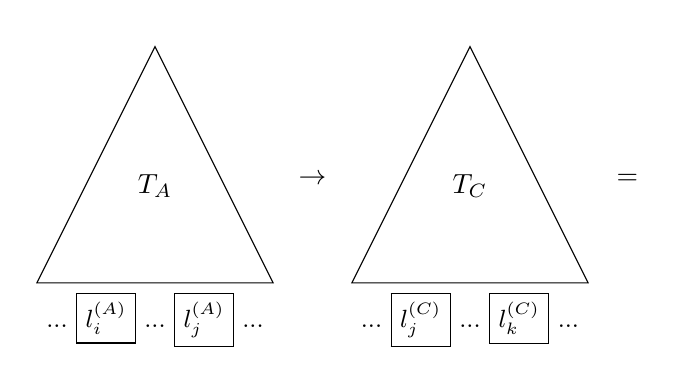
\begin{tikzpicture}
			\draw (1.5,1.5) node[anchor=north]{$T_A$};
			\draw (1.5,0) node[anchor=north]{\small$... \ \fbox{$l^{(A)}_i$} \ ... \ \fbox{$l^{(A)}_j$} \ ...$};
			\draw (0,0) node[anchor=north]{}
			-- (3,0) node[anchor=north]{}
			-- (1.5,3) node[anchor=south]{}
			-- cycle;
			\draw (3.5,1.5) node[anchor=north]{$\rightarrow$};
			\draw (5.5,1.5) node[anchor=north]{$T_C$};
			\draw (5.5,0) node[anchor=north]{\small$... \ \fbox{$l^{(C)}_j$} \ ... \ \fbox{$l^{(C)}_k$} \ ...$};
			\draw (4,0) node[anchor=north]{}
			-- (7,0) node[anchor=north]{}
			-- (5.5,3) node[anchor=south]{}
			-- cycle;
			\draw (7.5,1.5) node[anchor=north]{$=$};
	\end{tikzpicture}}
	\scalebox{.7}{
		\begin{tikzpicture}
			\draw (4,5.5) node[anchor=north]{$T_A$};
			\draw (4,4) node[anchor=north]{\small$... \ \dbox{$l^{(A)}_i$} \ ................................. \ \dbox{$l^{(A)}_j$} \ ...$};
			\draw (1,4) node[anchor=north]{}
			-- (7,4) node[anchor=north]{}
			-- (4,7) node[anchor=south]{}
			-- cycle;
			\draw (1.25,1.5) node[anchor=north]{$T_C \cap l^{(A)}_i$};
			\draw (1,0) node[anchor=north]{\footnotesize$l^{(C)}_i\cap l^{(A)}_i \ ... \ \fbox{$l^{(C)}_j \cap l^{(A)}_i$} \ ... \ \fbox{$l^{(C)}_k \cap l^{(A)}_i$}$};
			\draw (-1.5,0) node[anchor=north]{}
			-- (3.5,0) node[anchor=north]{}
			-- (1.75,3) node[anchor=south]{}
			-- cycle;
			\draw (6.75,1.5) node[anchor=north]{$T_C \cap l^{(A)}_j$};
			\draw (7,0) node[anchor=north]{\footnotesize$l^{(C)}_i \cap l^{(A)}_j \ ... \ \fbox{$l^{(C)}_j \cap l^{(A)}_j$} \ ... \ \fbox{$l^{(C)}_k \cap l^{(A)}_j$}$};
			\draw (4.5,0) node[anchor=north]{}
			-- (9.5,0) node[anchor=north]{}
			-- (6.25,3) node[anchor=south]{}
			-- cycle;
	\end{tikzpicture}}
	\caption[]{Schema of the derivation of a conditional Qtree. Nodes in \setlength{\fboxsep}{1pt}\dbox{dashed boxes} refer to the nodes that were verifying in the input antecedent Qtree, but are no longer verifying in the output conditional Qtree. Nodes in \setlength{\fboxsep}{1pt}\fbox{solid boxes} refer to the nodes that were verifying in the input consequent Qtree, and are thus still verifying in the output conditional Qtree.}\label{fig2:conditional-qtree-schema}
\end{figure} 


Second, the Node-Qtree intersection operation ($N\cap T$), which is part of the conditional Qtree formation process, is ``vacuous'' iff $N$ entails a specific leaf in $T$. We call the operation $N \cap T$ vacuous if it outputs $N$; the status of $N$ as verifying still depends on $T$'s verifying nodes. This is exemplified in Figure (\ref{fig2:vacuous-tree-node-inter}) assuming the node $N$ intersecting the Qtree entails (i.e. is a subset of) the leaf labeled $L$ in $T$. What happens is the following. The definition of a Qtree (see (\ref{ex2:qtree-def})) states that each intermediate node is partitioned by the set of its children. A corollary of this definition, is that, given a leaf $L$, all the nodes present on the path from $L$ to the root will be supersets of $L$, while all the other nodes will have no overlap with $L$. So, if $N \subseteq L$, $N$ will be a subset of all the nodes in $L$'s path to the root, and have no overlap with the other nodes, as well. Performing $N \cap T$ will thus initially yield a tree with same structure as the input Qtree $T$, but with nodes equal to $N$ along the path between the root and $L$'s original position, and empty nodes in all other positions. The Qtree reduction process devised in (\ref{ex2:qtree-reduction}) then removes all these empty nodes, and collapses the path made of $N$-nodes into one single node, namely, $N$. The whole operation therefore returns the input node $N$. Because the status of being a verifying node percolates when reduction takes place, as per (\ref{ex2:n-t-inter}), the output $N$ will be verifying iff $L$ was in $T$.



\begin{figure}[H]
	\centering
	\begin{minipage}[c]{.45\linewidth}
		\centering
		\begin{forest}
			[N$\cap$A[N$\cap$B[N$\cap$E][N$\cap$F]][N$\cap$C][N$\cap$D[N$\cap$G[N$\cap$J][N$\cap$K][N$\cap$L]][N$\cap$H][N$\cap$I]]]
		\end{forest}
	\end{minipage}
	\begin{minipage}[c]{.05\linewidth}
		\centering
		$\stackrel{N \subseteq K}{=}$
	\end{minipage}
	\begin{minipage}[c]{.25\linewidth}
		\centering
		\begin{forest}
			[N[$\emptyset$[$\emptyset$][$\emptyset$]][$\emptyset$][N[N[$\emptyset$][$\emptyset$][N]][$\emptyset$][$\emptyset$]]]
		\end{forest}
	\end{minipage}
	\begin{minipage}[c]{.1\linewidth}
		\centering
		$\stackrel{(\text{\ref{ex2:qtree-reduction}})}{=}$ N
	\end{minipage}
	\caption{Vacuous Node-Qtree intersection if $N$ entails a leaf of $T$, e.g. $K$.}\label{fig2:vacuous-tree-node-inter}
\end{figure}

The whole conditional Qtree formation process will then be vacuous if each verifying leaf in the antecedent Qtree entails a specific leaf of the consequent Qtree. Moreover, if each verifying leaf in the antecedent Qtree entails a specific \textit{non-verifying} leaf of the consequent Qtree, the output Qtree will be structurally identical to the antecedent Qtree but, will be left with \textit{no} verifying node. Such a tree will be deemed ill-formed as per principle (\ref{ex2:vacuous-flagging}). \\

We are now equipped to build conditional Qtrees from the sentences $S_{p}$=\textit{Ido is at SuB}, $\neg S_{p}$=\textit{Ido is not at SuB}, $S_{q}$=\textit{Ido is in Cambridge}, and $\neg S_{q}$=\textit{Ido is not in Cambridge}, whose Qtrees where computed in the previous Sections. This is done for $\neg S_p \rightarrow S_q$ in Figure \ref{fig2:qtrees-nptq}, using Qtrees for $\neg S_p$ from Figure \ref{fig2:qtrees-np} and Qtrees for $S_q$ from Figure \ref{fig2:qtrees-q}. Figure \ref{fig2:qtrees-nqtp}, does the same for $\neg S_q \rightarrow S_p$, just swapping the roles of $p$ and $q$. It is worth noting that the Qtrees in Figure (\ref{fig2:qtree-nptq-wh}) and (\ref{fig2:qtree-nqtp-wh}) are structurally identical to the antecedent Qtree used to build them. Such Qtrees are thus examples of a vacuous application of the Node-Qtree intersection operation. Their verifying nodes are however different from those of their antecedent Qtree, since, by definition, they are inherited from their consequent Qtree. 

\begin{figure}[H]
	\centering
	\begin{subfigure}[b]{.3\linewidth}
		\centering
		\scalebox{1}{
			\begin{forest}
				[CS [{$\p$}][\dbox{$\neg \p$} [\fbox{$\q$}][$\neg \q \cap \neg \p$]]]
			\end{forest}
		}
		\caption{Figure (\ref{fig2:qtree-np-polar}) $\rightarrow$ Figure (\ref{fig2:qtree-q-polar})}\label{fig2:qtree-nptq-polar-polar}
	\end{subfigure}\hfill
	\begin{subfigure}[b]{.3\linewidth}
		\centering
		\scalebox{1}{
			\begin{forest}
				[CS [{$\p$}][\dbox{$\neg \p$} [\fbox{$\q$}][$\r$][...]]]
			\end{forest}
		}
		\caption{Figure (\ref{fig2:qtree-np-polar}) $\rightarrow$ Figure (\ref{fig2:qtree-q-wh})}\label{fig2:qtree-nptq-polar-wh}
	\end{subfigure}\hfill
	\begin{subfigure}[b]{.3\linewidth}
		\centering
		\scalebox{1}{
			\begin{forest}
				[CS [{$\p$}][\fbox{$\q$}][\dbox{$\r$}][\dbox{...}]]
			\end{forest}
		}
		\caption{Figure (\ref{fig2:qtree-np-wh}) $\rightarrow$ Figure (\ref{fig2:qtree-q-polar})/(\ref{fig2:qtree-q-wh})\footnotemark}\label{fig2:qtree-nptq-wh}
	\end{subfigure}
	\caption[]{Qtrees for $\neg S\protect_{\p} \rightarrow S\protect_{\q} =$ \textit{If Ido is not at SuB then he is in Cambridge}. Nodes in \setlength{\fboxsep}{1pt}\dbox{dashed boxes} refer to the nodes that were verifying in the input antecedent Qtree, but are no longer verifying in the output conditional Qtree. Nodes in \setlength{\fboxsep}{1pt}\fbox{solid boxes} refer to the nodes that were verifying in the input consequent Qtree, and are thus still verifying in the output conditional Qtree.}
	\label{fig2:qtrees-nptq}
\end{figure}
\footnotetext{This Qtree is derived \textit{via} intersection and reduction as defined in (\ref{ex2:n-t-inter}). The Qtree derived \textit{before} reduction is given in (\ref{fig2:qtree-nptq-wh-before-reduc}). Reduction on this Qtree collapses the two $q$-nodes and makes the resulting node verifying; collapses the two $r$-nodes and makes the resulting node non-verifying; and so on for all other nodes different from the $p$-node.
	\begin{exe}
		\ex {\scalebox{.6}{
				\begin{forest}
					[CS [{$p$}][\dbox{$q$} [\fbox{q}]][\dbox{$r$} [r]][\dbox{...} [...]]]
		\end{forest}}}\label{fig2:qtree-nptq-wh-before-reduc}
	\end{exe}
}\label{fn:qtree-reduc}

\begin{figure}[H]
	\centering
	\begin{subfigure}[b]{.3\linewidth}
		\centering
		\scalebox{1}{
			\begin{forest}
				[CS [{$\q$}][\dbox{$\neg \q$} [\fbox{$\p$}][$\neg \p \cap \neg \q$]]]
			\end{forest}
		}
		\caption{Figure (\ref{fig2:qtree-nq-polar}) $\rightarrow$ Figure (\ref{fig2:qtree-p-polar})}\label{fig2:qtree-nqtp-polar-polar}
	\end{subfigure}\hfill
	\begin{subfigure}[b]{.3\linewidth}
		\centering
		\scalebox{1}{
			\begin{forest}
				[CS [{$\q$}][\dbox{$\neg \q$} [\fbox{$\p$}][$\r$][...]]]
			\end{forest}
		}
		\caption{Figure (\ref{fig2:qtree-nq-polar}) $\rightarrow$ Figure (\ref{fig2:qtree-p-wh})}\label{fig2:qtree-nqtp-polar-wh}
	\end{subfigure}\hfill
	\begin{subfigure}[b]{.3\linewidth}
		\centering
		\scalebox{1}{
			\begin{forest}
				[CS [{$\q$}][\fbox{$\p$}][\dbox{$\r$}][\dbox{...}]]
			\end{forest}
		}
		\caption{Figure (\ref{fig2:qtree-nq-wh}) $\rightarrow$ Figure (\ref{fig2:qtree-p-polar})/(\ref{fig2:qtree-p-wh})}\label{fig2:qtree-nqtp-wh}
	\end{subfigure}
	\caption[]{Qtrees for $\neg S\protect_{\q} \rightarrow S\protect_{\p} =$ \textit{If Ido is not in Cambridge then he is at SuB}; obtained \textit{mutatis mutandis} from Figure \ref{fig2:qtrees-nptq}}
	\label{fig2:qtrees-nqtp}
\end{figure}

At that point, we can already observe that Qtrees built from $\neg S_{p} \rightarrow S_q$, do not flag the $p$-node as verifying, since this corresponds to falsifying the antecedent of the conditional, a strategy that is typically overlooked. This feature of the model will be crucial in deriving the felicity of (\ref{ex2:pv(nptq)}): because $p$ is not treated as verifying in the Qtrees in Figure \ref{fig2:qtrees-nptq}, it will be possible to disjoin them with a Qtree for $S_p$, without producing redundant Qtrees as output. To clarify this intuition, we proceed to defining disjunction over Qtrees.




\subsection{Questions evoked by disjunctive LFs}
Building on \cite{Simons2001,Zhang2022}, we assume disjunctive LFs evoke questions pertaining to both disjuncts \textit{in parallel}. In other words, disjuncts should mutually address each-other's questions. This is modeled in (\ref{ex2:disj-qtree}), by assuming that disjunctions return all possible unions of the Qtrees evoked by both disjuncts, filtering out the outputs that do not qualify at Qtrees.

\begin{exe}
	\ex {\textit{Qtrees for disjunctive LFs.} A Qtree $T$ for $X \vee Y$ is obtained from a Qtree $T_X$ for $X$ and a Qtree $T_Y$ for $Y$ by:
		\begin{itemize}
			\item unioning the nodes, edges, and verifying nodes of $T_X$ and $T_Y$;
			\item returning the output only if it is a Qtree.
		\end{itemize}
		In other words, $Qtrees(X \vee Y) = \lbrace T_X \cup T_Y | T_X \cup T_Y \text{verifies (\ref{ex2:qtree-def})} \wedge (T_X, T_Y) \in Qtrees(X) \times Qtrees(Y) \rbrace$}\label{ex2:disj-qtree}
\end{exe}

A prediction of this definition is that two Qtrees sharing the same CS can be properly disjoined only iff they appear structurally parallel up to a certain level, and any further partitionings they independently introduce do not ``clash'' with each other.\footnote{We assume two Q-trees $T$ and $T'$ feature a bracketing clash iff there is $N \in T$ and $N' \in T'$ s.t. $N=N'$ but the sets of children of $N$ and $N'$ differ. We show that if $T$ and $T'$ exhibit such a clash, their disjunction is not a Q-tree. Let's call $C$ and $C'$ the sets of nodes of resp. $T$ and $T'$ that induce a bracketing clash; by assumption, $C$ and $C'$ are s.t. $C\neq C'$, and have mothers $N$ and $N'$ s.t. $N=N'$. Because $\vee$ achieves graph-union, $T\vee T'$ will have a node $N$ with $C\cup C'$ as children, and because $C\neq C'$, $C\cup C' \supset C, C'$. Given that both $C$ and $C'$ are partitions of $N$, $C\cup C'$ cannot be a partition of $N$. Conversely, if two Q-trees $T$ and $T'$ sharing the same CS as root are s.t. their union $T \cup T'$ is not a Qtree, it must be because $T$ and $T'$ had a bracketing clash. Indeed, under those assumptions, $T \cup T'$ not being a Qtree means one node $N$ in $T \cup T'$ is not partitioned by its children. Given $N$ is in $T \cup T'$, $N$ is also in $T$, $T'$, or both. If $N$ was only in, say, $T$, then it means $N$'s children are also only in $T$, but then, $T$ itself would have had a node not partitionned by its children, contrary to the assumption $T$ is a Qtree. The same holds \textit{mutatis mutandis} for $T'$, so, $N$ must come from \textit{both} $T$ and $T'$. Let us call $C$ and $C'$ the partitioning introduced by $N$ in resp. $T$ and $T'$. The fact $C$, $C'$, but not $C \cup C'$ partition $N$ entails $C\neq C'$, i.e. $T$ and $T'$ feature a bracketing clash.}

The only possible Qtree for $S_p \vee S_q$ / $S_q \vee S_p$ is given in Figure \ref{fig2:qtree-pvq}. It is obtained from Qtrees \ref{fig2:qtree-p-wh} and \ref{fig2:qtree-q-wh}, which, as previously observed, have similar structures. As intuitively expected, it is a Qtree that inquires about $p$ and about $q$ \textit{at the same time} (i.e., as part of the same subquestion), since the $p$ and $q$ nodes appear at the same level of the tree. Other possible unions of Qtrees are shown in Figure \ref{fig2:qtree-pvq-ill-formed} but appear ill-formed, because the leaves of such Qtrees do not properly partition the CS. Following a similar line of reasoning, one can use the Qtrees in Figures \ref{fig2:qtree-p-wh} (for $p$) and \ref{fig2:qtree-pvq} (for $p\vee q$), to derive the only possible Qtree for (\ref{ex2:pv(pvq)-repeated}) = $p\vee(p\vee q)$. Because Qtrees \ref{fig2:qtree-p-wh} and  \ref{fig2:qtree-pvq} have same structure, and are s.t. the former Qtree's set of verifying nodes is a subset of the latter Qtree's set of verifying nodes, Qtree union simply returns Qtree \ref{fig2:qtree-pvq} as output. So Qtree \ref{fig2:qtree-pvq} turns out to be compatible with both $p \vee q$ and (\ref{ex2:pv(pvq)-repeated}).

\begin{figure}[H]
	\centering
	\scalebox{1}{
		\begin{forest}
			[CS [\fbox{$\p$}] [\fbox{$\q$}] [\r] [...]]
		\end{forest}
	}
	\caption{Only well-formed Qtree evoked by $S\protect_{\p} \vee S\protect_{\q} =$ \textit{Ido is at SuB or in Cambridge}, obtained from Qtrees \ref{fig2:qtree-p-wh} and \ref{fig2:qtree-q-wh}. \textbf{This Qtree is also the only Qtree compatible with (\ref{ex2:pv(pvq)-repeated})}.}\label{fig2:qtree-pvq}
\end{figure}

Figure (\ref{fig2:qtree-pvq}) already gives us a hint as to why (\ref{ex2:pv(pvq)-repeated}) is degraded: there is an expression, namely $p \vee q$, that is strictly simpler than (\ref{ex2:pv(pvq)-repeated}) (and in fact, a proper simplification of (\ref{ex2:pv(pvq)-repeated})), that accommodates the exact same Qtree (including verifying nodes). In that sense, (\ref{ex2:pv(pvq)-repeated}) appears suboptimal. This will be formalized in the next Section.


\begin{figure}[H]
	\centering
	\begin{subfigure}[b]{.3\linewidth}
		\centering
		\scalebox{1}{
			\begin{forest}
				[CS [\fbox{$\p$}][\textcolor{red}{$\neg \p$}][\fbox{\q}][\r][...]]
			\end{forest}
		}
		\caption{Figure \ref{fig2:qtree-p-polar} $\vee$ Figure \ref{fig2:qtree-q-wh}}
	\end{subfigure}\hfill
	\begin{subfigure}[b]{.3\linewidth}
		\centering
		\scalebox{1}{
			\begin{forest}
				[CS [\fbox{$\q$}][\textcolor{red}{$\neg \q$}][\fbox{\p}][\r][...]]
			\end{forest}
		}
		\caption{Figure \ref{fig2:qtree-p-wh} $\vee$ Figure \ref{fig2:qtree-q-polar} }
	\end{subfigure}\hfill
	\begin{subfigure}[b]{.3\linewidth}
		\centering
		\scalebox{1}{
			\begin{forest}
				[CS [\textcolor{red}{\fbox{$\q$}}][\textcolor{red}{$\neg \q$}][\fbox{\p}][$\neg \p$]]
			\end{forest}
		}
		\caption{Figure \ref{fig2:qtree-p-polar} $\vee$ Figure \ref{fig2:qtree-q-polar}}
	\end{subfigure}
	\caption{Ill-formed Qtrees resulting from the union of the Qtrees in Figures \ref{fig2:qtrees-p} and \ref{fig2:qtrees-q}. \textcolor{red}{Red} nodes are nodes that should be removed for the leaves to form a proper partition of the CS.}
	\label{fig2:qtree-pvq-ill-formed}
\end{figure}







